% !Mode:: "TeX:UTF-8"
% !TEX root = ..\thesis.tex
\chapter{研究对象现状与分析}
本文以某汽车电子有限公司的装配车间为研究对象,进行调研。本章将介绍该公司车间的基本情况,并对现有装配线调度情况进行初步分析,指出现有计划安排和调度存在的主要问题,然后针对这些问题,提出合理改进方案。

\section{公司基本情况}
该汽车电子有限公司主要产品为车用电子电器开关、控制模块、控制面板等,是美国通用、德国大众、一汽大众、上海大众等国内外40余家汽车主机厂的专业定点配套供应商,配套的代表性车型有奥迪A6(L)、奥迪A4(L)、奥迪Q5、捷达等系列轿车,以及卡车、轻型车、微型车等,产品型号达6000余种。

该公司的订单特点是品种多、批量大、小型产品、工艺成熟,所以采用流水线生产是比较合适的,与其合作较多的客户(主机厂)一般有其专用线,专门负责该主机厂的订单生产。订单从接受到交付的流程如\reff{fig:orderflow}所示,其中虚线框内为装配车间的作业。在没有订单或者订单较少时,为了不让生产线停下来,需要进行工厂内部的计划生产,而订单较多时需要加班作业。
\begin{figure}[h]
\centering
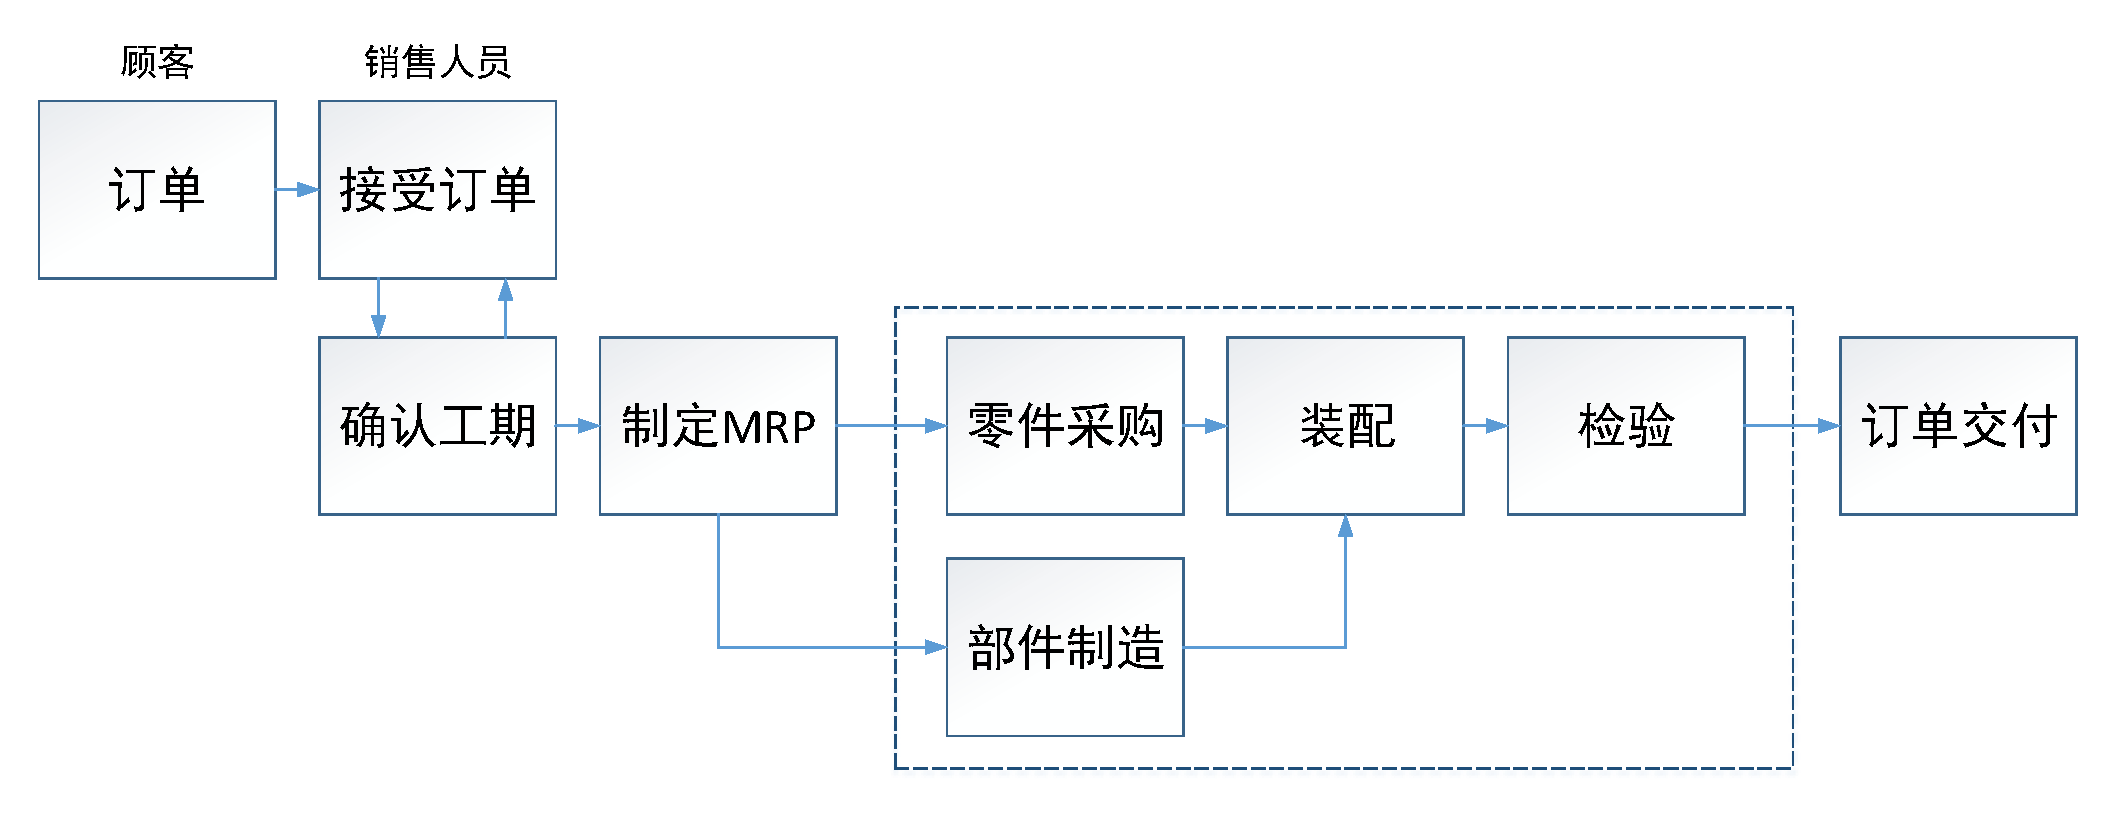
\includegraphics[width = 13cm]{orderflow.pdf}
\caption{现行订单信息流\label{fig:orderflow}}
\end{figure}
\section{装配车间作业}
该公司的制造部分为制造一部和制造二部,制造一部主要是负责零部件的生产,不是本课题的主要研究对象;制造二部主要是负责产品总装,共8个车间,均是流水线作业,是本课题的研究对象,其相关信息如\reft{tab:2jobshopinfo}所示(单位:个)。
\begin{table}[htbp]
  \centering
  \caption{制造二部装配车间信息}
    \begin{tabular}{cccccccccc}
    \toprule
    \multicolumn{2}{c}{车间 } & 1车间   & 2车间   & 3车间   & 4车间   & 5车间   & SGM车间 & 通用车间  & 电子车间 \footnote{包括:模块线、插件线及SMT线三个部分,其中,模块线是总装线,共5条装配线,插件线和SMT线是零部件生产线。本次研究的重点是总装线,故电子车间只列出了部分信息。} \\
    \midrule
    \multicolumn{2}{c}{班 组 数 量} & 6     & 6     & 6     & 5     & 4     & 4     & 6     & 2 \\
    \multicolumn{2}{c}{流水线数量} & 7     & 7     & 7     & 6     & 7     & 6     & 5     & 5 \\
    \multicolumn{2}{c}{PMC分配品种数} & 777   & 557   & 186   & 196   & 334   & 29    & 76    & 83 \\
    \bottomrule
    \end{tabular}
  \label{tab:2jobshopinfo}
\end{table}

每个总装车间均有多条生产流水线,为方便管理,每条流水线负责各自对应主机厂的装配生产。当主机厂需要多个品种的产品时,流水线根据订单顺序进行装配作业,即同一主机厂的产品在一条生产线上轮流生产。


\section{产线调度现状}
当前该公司装配车间采用专线生产的方式,即客户的订单在其专用的流水线上进行生产作业,当同一客户有多个订单下达时,按照先到先服务(FCFS)的规则进行装配生产安排,多条产线并行作业互不干扰。

订单或任务到达时,如果有流水生产线空闲可用,则立刻对其根据进行生产准备,然后开始装配生产。若产线在处理订单,那么将该订单安排入其专线队列中,等待前面的批量订单生产完毕再进行生产。现行调度的产线如\reff{fig:3nowschedule}\footnote{\reff{fig:3nowschedule}中订单a -- b 表示主机厂a 的第b 个订单,下同}所示。
\begin{figure}[h]
\caption{$3$条生产线的现行调度\label{fig:3nowschedule}}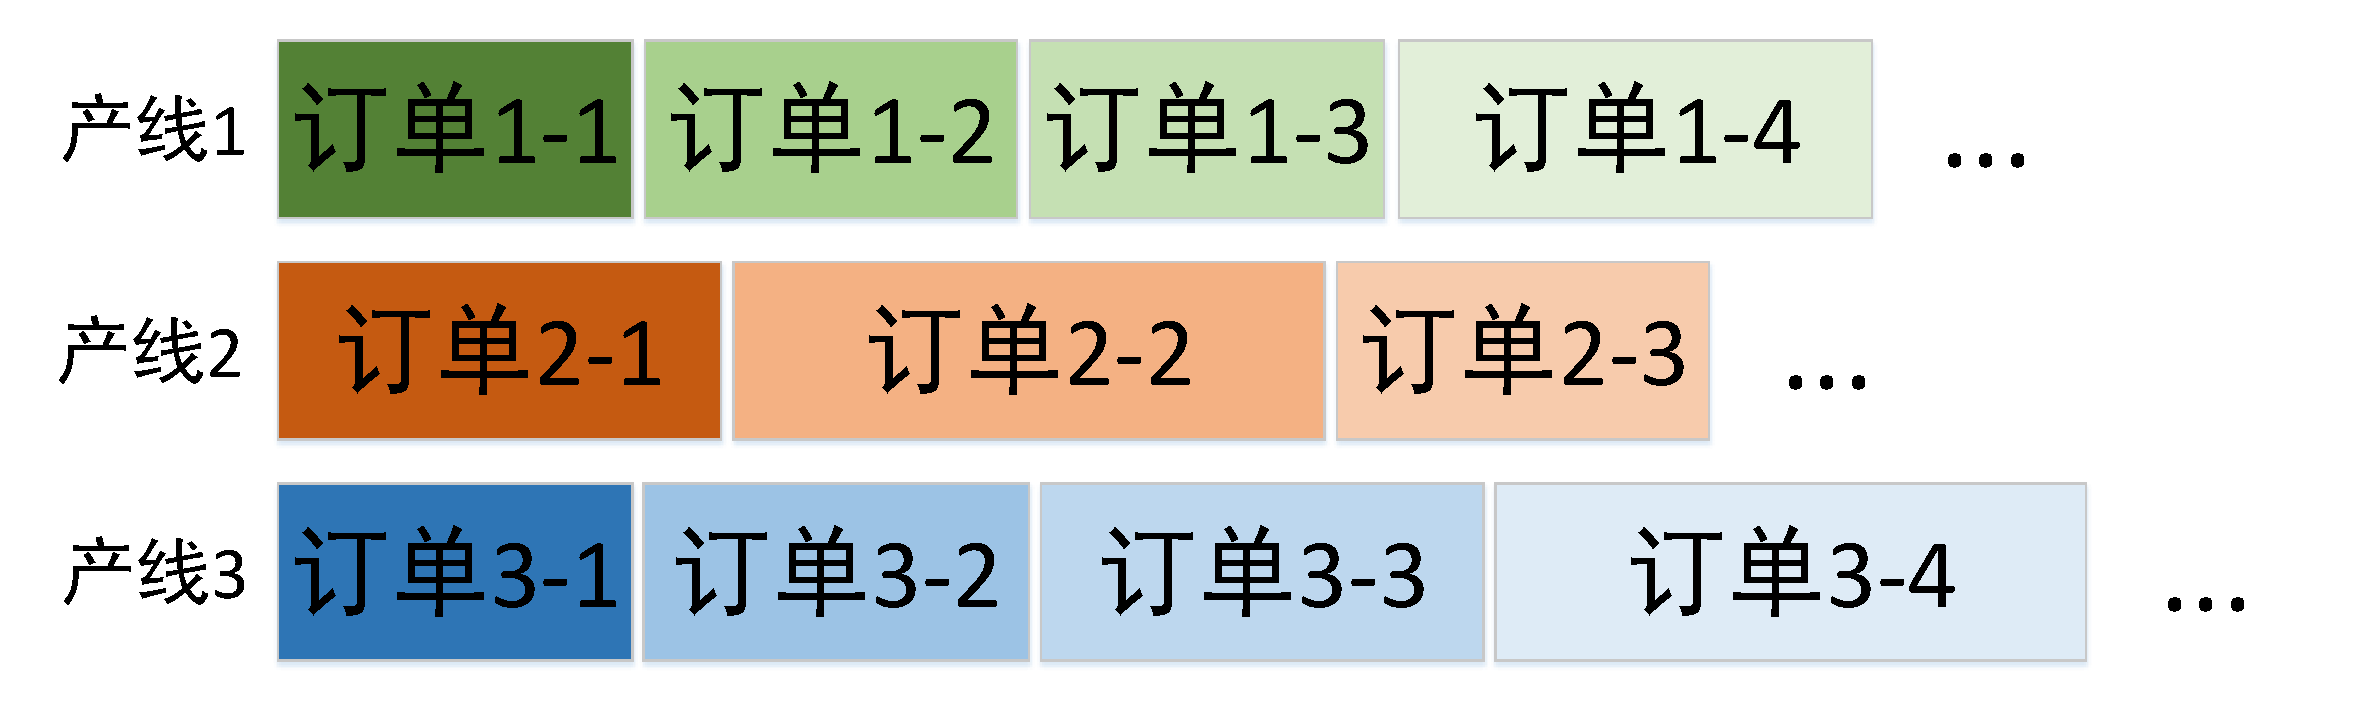
\includegraphics[width = 8cm]{orderschedulenow.pdf}
\end{figure}

现行调度方法逻辑简单,执行力强,每条装配线可分时生产不同品种的产品,而且按照厂家来安排组织生产,方便了管理。然而其缺陷也是明显的,例如常常会产生有些产线队列很长而有限产线空闲无作业,造成极大浪费。具体的现有问题将在下一章分析。


\section{生产线分析}
课题研究对象是该汽车电子公司的总装生产线,是典型的流水车间,每条流水线负责同一主机厂的不同品种产品总装流程。装配生产根据订单批量进行安排,根据先到先服务(FCFS)规则生成任务队列。

生产线分析包括上述这些差别及其产生的影响或效果,具体描述从订单、装配到交付的流程,并分析现行调度方案的一些指标。

\subsection{现行流程描述}
现行下达订单到交付的流程如\reff{fig:orderflow}所示,销售人员接到客户订单,在确认工期后,将之送达计划部门,制定主生产计划(MRP),随后根据产品特性安排采购与厂内加工。根据任务队列与批量进行产品总装,通过质检包装后,销售人员安排运输送达至客户。
订单到达会立即安排入其对应的主机厂专用产线,当同一主机厂有多个订单同时到达时,则根据最早交货期(EDD)规则进行生产调度。

本课题的研究对象是流程中的总装调度安排,......................
\subsection{现行调度方案}
任务下达到车间时,需要根据订单队列及其批量进行调度安排,....................
现行调度方案逻辑简单,执行力强,每条装配线可分时生产不同品种的产品,而且按照厂家来安排组织生产,方便了管理。
\subsection{主要问题}
现行调度方案存在诸多问题,例如多条装配线负荷不均衡,有的任务过重,有的任务不足,负荷不均衡,一条装配线上装配的产品工艺相似性较低,导致换线时间增加,产生更长的等待。

根据现行调度情况进行问题分析,可以归纳其主要存在问题如下:
\renewcommand{\labelenumi}{(\theenumi)}
\begin{asparaenum}
\item 产线利用率低
\suspend{asparaenum}

产线利用率低主要体现在存在大量换线时间,一方面由于产线等待队列由FCFS 规则产生,同时到达的订单也只是根据EDD 规则安排,没有考虑品种装配流程间的相似性。当这种差异很大时,必然会增加换线时间,进而增加了任务间的等待。另一方面,由于产线的专用性,当有多条产线都能处理某个任务时,该任务只能在订单来自的主机厂专线上生产,闲置了可用线的生产能力。
\resume{asparaenum}
\item 生产不均衡
\suspend{asparaenum}

这里的生产均衡和混流生产中的均衡生产稍有差别,此处的不均衡现象更为宏观。来自不同主机厂的任务在不同产线上进行处理,这样一来,订单较多、较频繁的主机厂产线总是会处于繁忙状态,而订单较少的产线则呈现为停线等待居多。这种不均衡现象直接导致产能的巨大浪费,同时也间接导致了换线时间增加,因为不均衡的生产业表面订单较为集中。突破专线限制可以解决宏观不均衡问题,虽然细分到单条线上的混流生产可以近一步均衡化生产,但其需要较高的管理投入,可以考虑折衷。
\resume{asparaenum}
\item 工艺及设备和生产需求不匹配
\suspend{asparaenum}

各流水线需要有多品种加工的能力,故线上需要有相应加工工艺的设备,而时常不同主机厂所需产品可能有很高的相似性,这使得同样的设备需要在多条流水线上设置,尤其对于加工时间较短、处理批量较少的作业,过多的设备徒增成本与闲置。另一方面,加工时间长、处理批量大的作业,较少的设备不利于生产效率,导致在制品增多。
\resume{asparaenum}
\item 工期可控性低
\suspend{asparaenum}

工期的可控性低主要体现在应变插单的问题上,现行调度采用的是不可中断的流水作业,各流水线只能按其队列顺序进行装配作业,由于这样安排没有顾及工期的先后即订单的具体情况,导致大部分订单都需要延期交货,也存在较多订单的过早完工,增加了库存。此外,虽然插单可以较为合理安排订单加工顺序,而然会带来额外的切换时间,需要权衡考虑。
\resume{asparaenum}
\item 产线冗余度高
\end{asparaenum}

前面几大问题已经涉及到了一些浪费现象,除了这些之外,该厂制造二部共有8个装配车间,每个装配车间有7--8条总装流水线,然而由于流水线是按主机厂进行分配,存在较高的冗余度,前面提到的产线间设备类似属于其中之一。产线的冗余还包括作业及管理人员,辅助设置,场地空间,相关能源等。

\section{方案改进}
上述问题为研究对象的目前的主要问题,并对其产生原因进行分析,这为改进调度方案明确了方向。
为制定合理调度方案,改善装配流水线现状,首先需要确定改进目标,进而根据目标的可行性,建立数学模型。
因此,本节将结合实际情况,权衡投入和效益,建立适合本课题研究对象的混线装配生产模型。
\subsection{改进设计}
目前的生产现状主要是存在各主机厂的专用流水线,所以首要的改进是突破专用线的生产界限。如此一来,生产线可以加工多家主机厂的订单,形成所谓的混线生产,是较混流生产为宏观的均衡化生产,如\reff{fig:orderschedule}所示
。其次,适当允许订单拆分到不同产线,安排插单作业,可以进一步改善现有浪费,而且增加生产应变能力。
\begin{figure}[h]
\centering
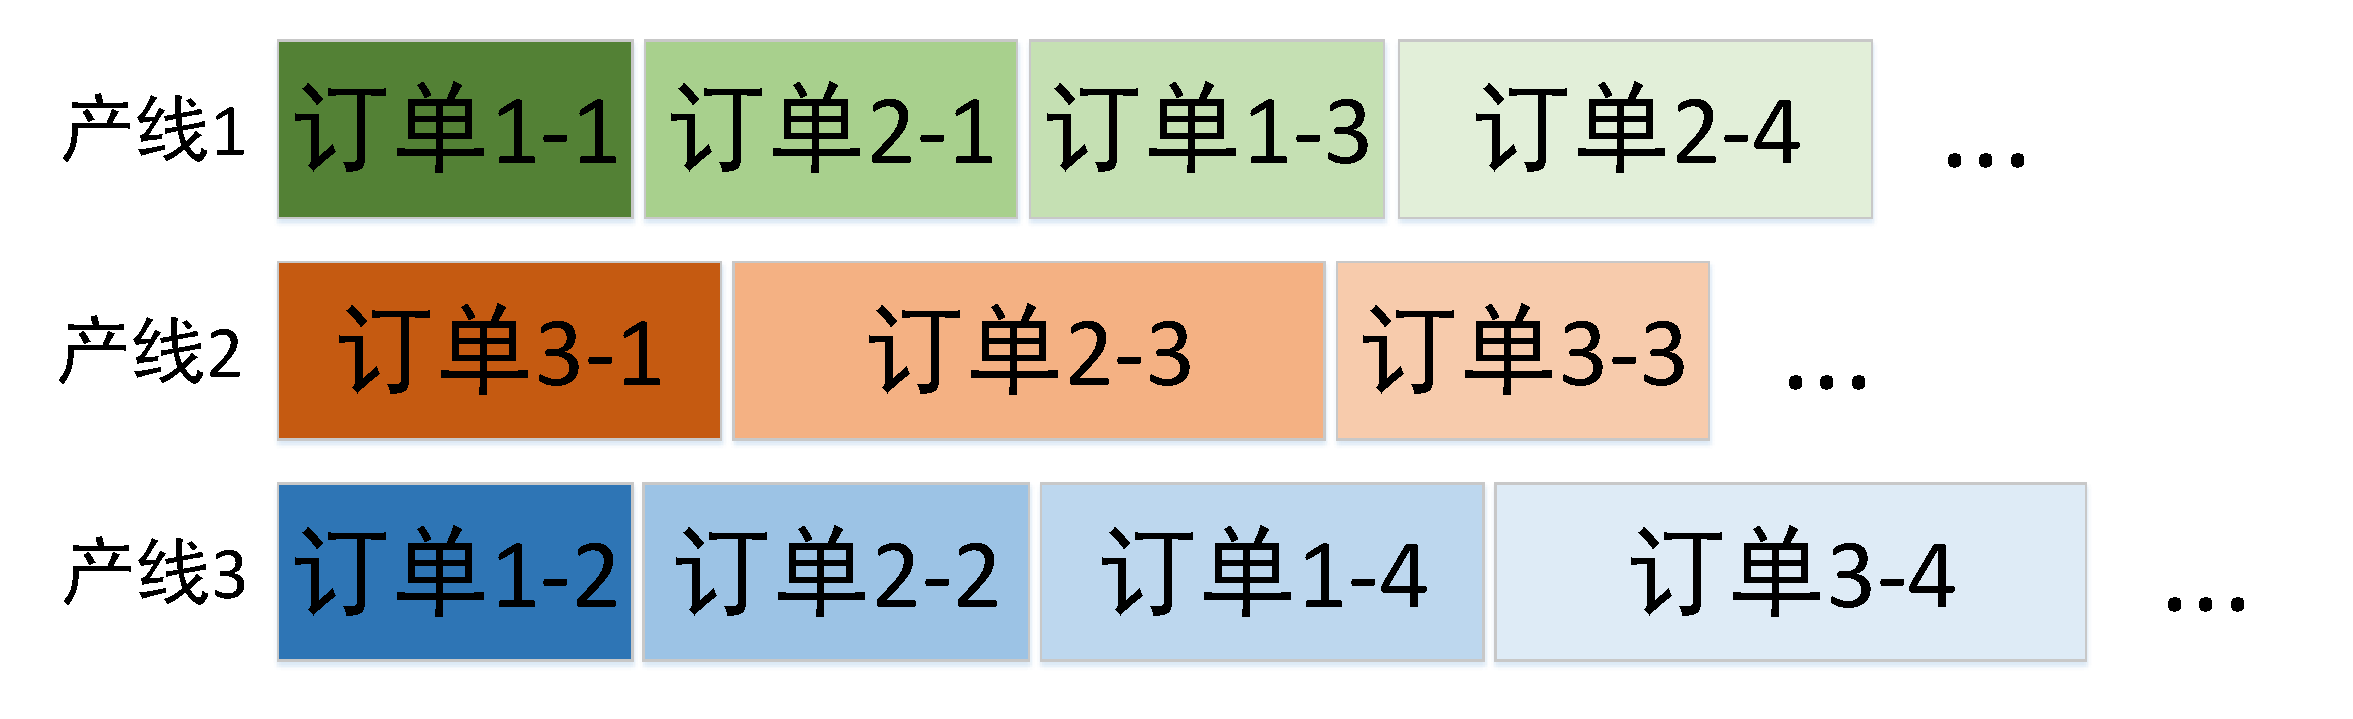
\includegraphics[width = 8cm]{oredrschedule.pdf}
\caption{$3$条产线的混线装配生产示意\label{fig:orderschedule}}
\end{figure}

\section{小结}
本章............
产线调度现状反映了一些问题,例如
